\documentclass[a4paper,reqno,oneside]{amsart} %amsbook ger en design mer lik den i boken, men är möjligen aningen för kompakt. article ger en mer luftig design med tydligare sektionsindelningar
%Options -- Point size:  10pt (default), 11pt, 12pt
%        -- Paper size:  letterpaper (default), a4paper, a5paper, b5paper
%                        legalpaper, executivepaper
%        -- Orientation  (portrait is the default)
%                        landscape
%        -- Print size:  oneside (default), twoside
%        -- Quality      final(default), draft
%        -- Title page   notitlepage, titlepage(default)
%        -- Columns      onecolumn(default), twocolumn
%        -- Equation numbering (equation numbers on the right is the default)
%                        leqno
%        -- Displayed equations (centered is the default)
%                        fleqn (equations start at the same distance from the right side)
%        -- Open bibliography style (closed is the default)
%                        openbib
% For instance the command
%           \documentclass[a4paper,12pt,leqno]{article}
% ensures that the paper size is a4, the fonts are typeset at the size 12p
% and the equation numbers are on the left side
%

\usepackage[activate={true,nocompatibility},final,tracking=true,kerning=true,spacing=true,factor=1100,stretch=10,shrink=10]{microtype}
\microtypecontext{spacing=nonfrench}
\usepackage{amsmath}%
\usepackage{amsfonts}%
\usepackage{amssymb}%
\usepackage{amsthm}
\usepackage{graphicx}
\usepackage[utf8]{inputenc}
\usepackage[english]{babel}
\usepackage{url}
\usepackage{color}
\usepackage{varioref}
\usepackage{epstopdf}

\usepackage[fixlanguage]{babelbib}
\selectbiblanguage{english}

\usepackage{comment}

\newtheorem{theorem}{Theorem}%[subsection]
\newtheorem{lemma}[theorem]{Lemma}
\newtheorem{cor}[theorem]{Corollary}

\theoremstyle{definition}
\newtheorem{definition}[theorem]{Definition}
\newtheorem{example}[theorem]{Example}
\newtheorem{xca}[theorem]{Exercise}

\theoremstyle{remark}
\newtheorem{remark}[theorem]{Remark}

\numberwithin{equation}{section}
%\renewcommand{\theequation}{\arabic{subsection}--\arabic{equation}}

\usepackage[toc,page]{appendix}

\newcommand{\abs}[1]{\left\lvert#1\right\rvert}
\newcommand{\R}{\mathbb{R}}
\newcommand{\Q}{\mathbb{Q}}
%\newcommand{\N}{\mathbb{N}}
\newcommand{\Z}{\mathbb{Z}}
\newcommand{\C}{\mathbb{C}}
\newcommand{\D}{\mathcal{D}}


%% Följande kod gör \emph fetstilt istället för kursiv
%\makeatletter
%\DeclareRobustCommand{\em}{%
%  \@nomath\em \if b\expandafter\@car\f@series\@nil
%  \normalfont \else \bfseries \fi}
%\makeatother

%% Följande kod gör att \Re och \Im skrivs som i boken istället för som gotiska kapitaler:

\renewcommand{\Re}[1]{\textrm{Re}(#1)}
\renewcommand{\Im}[1]{\textrm{Im}(#1)}

%% Skapar ett kommando för komplexa konjugatet:

\newcommand*\conj[1]{\overline{#1}}

%% Skapar ett kommando \grad för graden av ett polynom

\newcommand{\grad}[1]{\operatorname{grad}#1}

%% Skapar ett kommando \st som ger en | med rymd omkring sig

\newcommand{\st}{\ \lvert\ }

%% Skapar ett kommando \seq{a}{k} som skriver {a_k}

\newcommand{\seq}[2]{\{#1_{#2}\}}

%% Skapar ett kommando \anm som skriver Anmärkning:

\newcommand{\anm}{\emph{Anmärkning: }}

%% Skapar kommandon \df, \dx, \dy, \dt, \du, \ds som skriver differentialer
\newcommand{\df}{\mathrm{d}f}
\newcommand{\dx}{\mathrm{d}x}
\newcommand{\dy}{\mathrm{d}y}
\newcommand{\dt}{\mathrm{d}t}
\newcommand{\du}{\mathrm{d}u}
\newcommand{\ds}{\mathrm{d}s}

%% Skapar kommando \arccot som skriver arccot
\newcommand{\arccot}{\operatorname{arccot}}

%% Skapar kommando \intx och \intt för integral m.a.p. x och t:
\newcommand{\intx}[1]{\int #1\ \dx} 
\newcommand{\intt}[1]{\int #1\ \dt} 

% Skapar kommandon för konsistent typ för slumpvariabler
\newcommand{\T}{\mathfrak{T}} 
\newcommand{\X}{\mathfrak{X}}
\newcommand{\N}{\mathfrak{N}}
\newcommand{\p}{\mathfrak{p}}
\newcommand{\Paths}{\mathbb{P}}

%% Lägger in en bunt autogenererad kod för figurerna
\usepackage{pgf,tikz}
\usepackage{mathrsfs}
\usetikzlibrary{arrows}

\usepackage{epigraph}
\usepackage{listings}

\usepackage{verbatim}

\usepackage[a4paper, total={5.5in, 8in}]{geometry}

\begin{document}
\lstset{language=matlab}

\definecolor{light-red}{rgb}{0.8,0,0}
\definecolor{light-blue}{rgb}{0,0,0.8}
\definecolor{pale-pink}{rgb}{1,0.95,0.95}
\definecolor{cream-white}{rgb}{1,0.99,0.99}
\definecolor{pure-white}{rgb}{1,1,1}
\definecolor{pale-green}{rgb}{0.6,0.89,0.68}
\title{Analysis of Rock Art 3D Scans and Generation of 2D Images}

%    Information for first author
\author{Vilhelm Agdur}
%    Address of record for the research reported here
%\address{Department of Mathematics, Louisiana State University, Baton
%Rouge, Louisiana 70803}
%    Current address
%\curraddr{Department of Mathematics and Statistics,
%Case Western Reserve University, Cleveland, Ohio 43403}
%\email{xyz@math.university.edu}
%    \thanks will become a 1st page footnote.
%\thanks{The first author was supported in part by NSF Grant \#000000.}


%    General info
%\subjclass[2000]{Primary 54C40, 14E20; Secondary 46E25, 20C20}

%\date{January 1, 2001 and, in revised form, June 22, 2001.}

%\dedicatory{This paper is dedicated to our advisors.}

%\keywords{Differential geometry, algebraic geometry}

\begin{abstract}
In research on rock art in Sweden, a novel approach for documentation is the use of 3D-scanners, as opposed to earlier two-dimensional manual documentation techniques. In order to facilitate effective visualisation and analysis of these scans, we develop an algorithm for extracting the relevant 2D-data and denoising the scans. Various specific filters are implemented to analyse and remove the particular types of noise encountered in the scans. The resulting 2D-images are found to be considerably superior to older two-dimensional documentation techniques.\end{abstract}

\maketitle

\section{Introduction}

The rock art in Tanum, which is what we are primarily concerned with here, is from the Bronze Age, and depicts many different motifs -- boats, humans, weapons, animals, and various ritualistic symbols. They are believed to have been carved at different times through the time period, and with differing techniques, but this has so far been hard to study.\cite{ling_bertilsson_2015} 

In particular, this difficulty stems from the fact that all documentation has been two-dimensional and already interpreted -- data on the varying depth of the carvings, and on their differing clarity, has been suppressed in the production of sketches, while rubbings simply do not have the quality to discern such details. In order to provide more objective and thorough documentation, and allow more sophisticated methods of studying this documentation, researchers introduced 3D-scanning techniques.

However, with this new form of documentation, the opposite problem arises -- the resulting data files are huge, and are not easy to handle or analyse other than by visual inspection. Specific information, such as the depth of carvings, cannot be naïvely extracted straight from the data files, and the 3D-scan, being so faithful reproductions of the original rock surface, are no easier to interpret than the rock surface itself.

In order to ameliorate this problem, image analysis techniques are necessary. Particularly, it is necessary to remove the large scale curving of the rock surface, finding instead a cloud of measurements of the deviation of points from the idealised overall rock surface. This point-cloud is then interpolated into a high-resolution 2D image, preserving all the information on the local structure of the rock, while removing extraneous large-scale structure. Various techniques can then be used to remove the noise introduced by the texture of the rock surface and by the smoothing and striation of the rock by the ice-age ice shelves.

This results in an image which can be more easily visually interpreted, and can have various filters applied to it to give objective assistance to the interpretation. For example, it is considerably easier to visually detect what is man-made and what is natural in the processed image than in the raw scans, which is useful for countering the natural human tendency to see more pattern in data than there really is.

The output images are also susceptible to more sophisticated statistical analyses, such as classification algorithms and perhaps even methods that could answer the questions about chronology, carving technique, and authorship which have hitherto been beyond reach. That this might be possible with the use of 3D data has been suggested in the past\cite{portugal}, but it does not appear to have been actually done so far.

\section{Theory}

3D-scans and similar 3D documentation techniques have previously been used to archive and study various types of rock art, from paintings in Wonderwerk cave, South Africa\cite{wonderwerk}, and the Grotta dei Cervi in Puglia, Italy\cite{gdeicervi}, and to carvings in Cumbria, England,\cite{cumbria} Parpallo, Spain,\cite{parpallo}, and Cap Blanc, France\cite{capblanc}. Generally, the purpose has been to provide a more objective type of documentation that can be accessed remotely, to give greater access to the material both to academics and to the public. Additionally, the scanning technology does not rely on direct contact with the rock surface, and is thus better from a preservation standpoint. Another use which has been suggested in the literature for 3D-scans of rock art is to monitor their erosion.\cite{erosion,portugal}

One particularly interesting use case of this technology is in the study in Cumbria, where a spiral pattern on a rock had previously been visually observed and photographed, but could not be consistently rediscovered on the rock surface itself. One rubbing was produced after many attempts that showed the spiral pattern, but other attempts to find it failed. In the study, they use a 3D scanner and some other techniques to study the rock surface, and find no evidence of any carved spiral. 3D-scannings can thus be useful not only to study rock art, but also to prove that there is no rock art, countering the natural tendency which the study notes for the human mind to see more pattern than there really is.

Despite this widespread interest in 3D-scans of rock art, one thing which has remained relatively understudied is appropriate ways of visualising and working with the resulting data. Usually, what is used is just a standard 3D-model viewing software, with artificial lighting, and screenshots of this are used as figures in print. One study which breaks this pattern is by Trinks, 2005\cite{trinks}, who applies a high pass filter to the 3D data to suppress its natural curvature, producing flat visualisations. The method developed there is used to good effect to visualise rock art on the standing stone \emph{Long Meg} in Cumbria by Diaz-Andreu, 2005\cite{longmeg}.

From the opposite direction, there has been some interest in the application of more sophisticated machine learning techniques to rock art data, but this has only been applied to photographs or drawings of rock art, not 3D scans. Thus, they have been vulnerable to the known inaccuracy, low quality, and subjectivity of drawings and, to a lesser degree, of photographs. These studies have focused exclusively on the classification of large amounts of different petroglyphs -- one approach used neural nets\cite{patrec,kohonen}, while another used a distance measure based on the Hough transform to quantify distances between different petroglyphs, clustering using this distance measure.\cite{towindexing}

We will proceed from this point in the literature, redeveloping a slightly more sophisticated version of Trinks' method, and develop some further methods to remove extraneous noise from the scans, providing more clear visualisations. The method is developed with an eye towards the potential application of machine learning techniques to not only classification but also to the above-mentioned questions of carving technique and chronology of rock art.

\section{Data and methods}
\subsection{Data}
The rock art documentation is catalogued in SHFA, the Swedish Rock Art Research Archives\cite{shfa}, and the specific 3D-scans are accessible through ``Sketchfab''\cite{sketchfab} as .stl-files. Other forms of documentation are hosted on the SHFA page itself.

The .stl-file contains data on vertices and faces of a 2D-surface in 3D-space, and are typically between 40MB and 800MB. In order to extract a point-cloud from these files, we use the open-source ``CloudCompare'' software\cite{cloudcompare}, which offers considerably faster processing than all other options we tried. The set of vertices are saved as a .csv-file, allowing further processing.

\subsection{Pre-processing}
The point-cloud is loaded into Matlab as a $3\times N$ matrix, where $N$ is the amount of vertices. As a first step, to find the optimal orientation of the surface -- or equivalently to find which direction in the point-cloud to consider to be ``upwards'' -- we apply a principal component analysis. We choose the first two principal components to be our spatial dimensions in the resulting image, and the third to be the height dimension.

Having thus transformed our point-cloud, we then fit a fifth-degree bivariate polynomial to the point-cloud, finding our idealised rock surface. The residuals of this fit are then the depth of carving in various spots. We thus replace the previous height-dimension with these residuals, getting a flattened rock surface with the large-scale shape of the rock surface removed.

The technique of polynomial-fitting results in some very small amount of comparatively very large outliers, which generally throw various later calculations off, so we then remove the most deviant $0.5\%$ of points. These are always on the edges of the scan, and so we are not removing any useful data in this step.

In order to get it to be proper image data, we interpolate an image from the resulting point-cloud, choosing its dimensions to have the larger edge be $10000$ pixels. The resulting images are generally no larger than 40MB, so we achieve significant compression without losing any of the information we are interested in.

Finally, we apply a slight high pass filter to further smoothen the image, and normalize the pixel value range, again killing the largest outliers.

\subsection{Various types of noise}

Due to the accuracy of the 3D-scanner used being far greater than the scale of the features we are interested in, there is no significant issue of ``blurriness'' or other measurement inaccuracies. However, the rock bed contains many types of abrasion or other non-human-created features which for our purposes are noise.

One of the largest-scale problematic features is that many scans contain large cracks, such as the one in figure \ref{fig:largecrack}. Fortunately, none of the features we are interested in stretch across these cracks, so we can simply cut the scan into several pieces along the cracks, using CloudCompare, and analyse these pieces separately. The extreme outliers can then unproblematically be filtered out by the same outlier-removal as is applied to remove the polynomial fit outliers. Doing this also cuts down on processing time, since each piece will be smaller and faster to analyse.

\begin{figure}[!htb]
\centering
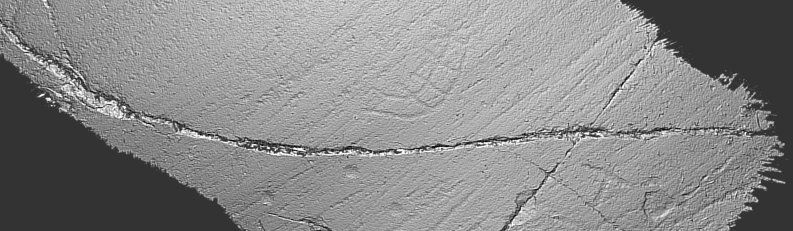
\includegraphics[scale=.5]{largecracks_t98_1.PNG}
\caption{A large crack, detail from Tanum 98:1}
\label{fig:largecrack}
\end{figure}

Another type of bad feature is medium-scale chipping, where pieces have been chipped off, as can be seen in a 3D scan and in a processed image in figure \ref{fig:mediumchip}. These are generally too similar to actual features to be filtered out by any simple method. They could be separated from features once identified by using the fact that they generally have much sharper edges and more convex shapes than the features we are interested in. This, however, would require at least some type of linear classifier, and is thus outside the scope of our project, and will not be considered further.

\begin{figure}[!htb]
\centering
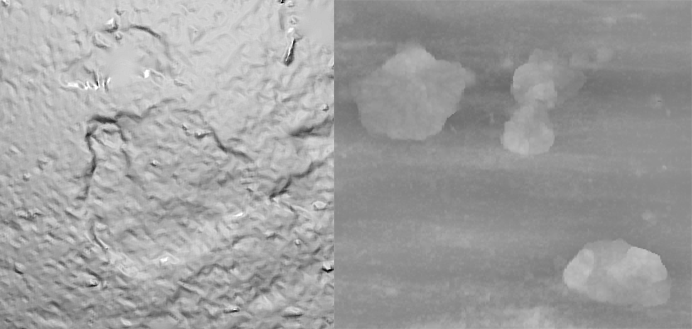
\includegraphics[scale=.5]{mediumchips.png}
\caption{A medium chip, left, detail from 3D of Tanum 98:1, right, detail from processed image of Tanum 94:1}
\label{fig:mediumchip}
\end{figure}


Another type of noise is the striation caused by the movement of the ice during the ice age -- this smoothed the rock surface, but, like a cheese-grater dragged in only one direction, introduced a new directional smaller scale structure on top of which later carvings and noise happened. This can be seen in a 3D-scan and in a processed image in figure \ref{fig:directed}.

This type of noise can be filtered out efficiently once the direction of the noise in the image has been identified, by a directional analogue of our previous high-pass filtering. Particularly, by applying a motion blur in the direction of the noise, subtracting the blurred image from the original, and normalising, the directional noise disappears. 

The main problem with this type of noise is rather that it is hard to accurately automatically detect the direction of this noise, and even harder to detect whether it is present in an image, due to it not introducing sharp lines but rather a continuous tendency. Thus it will, for best results, be necessary with human input to specify whether it is present, and if so in what direction it runs.

One tentative algorithm for determining its direction can however be specified as follows
\begin{enumerate}
    \item Binarize the image using adaptive thresholding
    \item Erode the resulting binary image slightly
    \item Remove small components, defined as components containing less than about two thousand pixels
    \item Take a Hough transform, identify the five biggest peaks, and take the direction of striation to be the mean of their angles
\end{enumerate}

This algorithm can give acceptable results, but does not perform as well as manual input. It may however be useful for bulk processing of a large amount of scans, where errors may be corrected manually afterwards.

\begin{figure}[!htb]
\centering
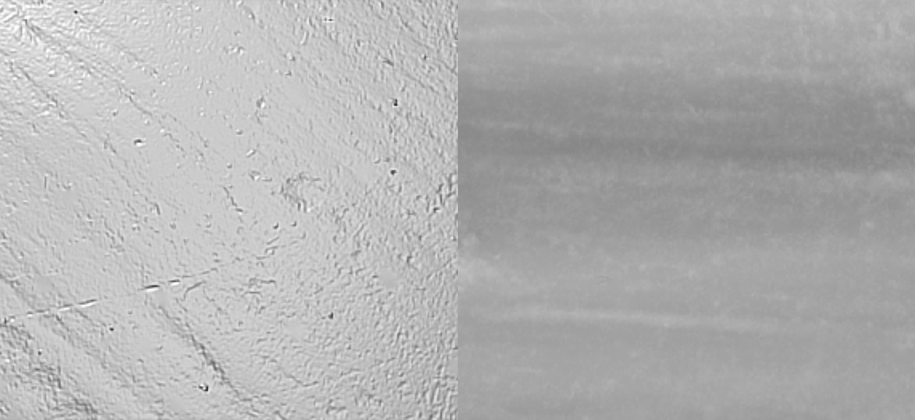
\includegraphics[scale=.35]{directed.png}
\caption{Some directional noise, left, detail from 3D of Tanum 99:1, right, detail from processed image of Tanum 94:1}
\label{fig:directed}
\end{figure}


Finally, there are some scans where the rock surface itself is not smoothed, or something has caused it to become irregular before or after carving. This can be seen in a 3D-scan and in a processed image of the same in figure \ref{fig:irregular}.

\begin{figure}[!htb]
\centering
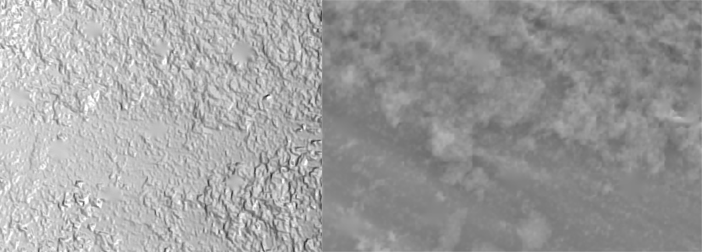
\includegraphics[scale=.5]{roughness_t113_1.png}
\caption{Irregular noise, detail from Tanum 113:1, in 3D, left, and in processed image, right}
\label{fig:irregular}
\end{figure}

\section{Results and conclusion}

\subsection{Result, comparison with other forms of documentation}

The resulting images are generally very satisfactory -- the desired features are clearly visible, and the image is homogeneous in contrast, indicating that the image has indeed been flattened. The noise introduced by striation is normally removed very accurately, revealing the features clearly. The superiority of this method to that of paper rubbings is obvious on comparison -- see, for example, figure \ref{fig:comparison}, which shows one rubbing, one coloured rubbing, one raw processed image, and one processed image with striation filtered out.

\begin{figure}[!htb]
\centering
\includegraphics[scale=.125]{comparisonfigure.png}
\caption{Comparison of four documentation types, all of Tanum 94:1.  Top-left: Processed and striation filtered out, top-right: processed but no striation filtering, bottom-left: coloured-in rubbing, bottom-right: uncoloured paper rubbing. Both rubbings also from SHFA.}
\label{fig:comparison}
\end{figure}

We can observe particularly that the removal of the striation has not affected the clarity of the features in the image, confirming that our filtering works as intended. In comparing with the uncoloured paper rubbing, we can see that we, as expected, get vastly higher resolution in the processed images, revealing especially the fainter features more clearly. We also find that the paper rubbing tends to be more ``binary'' -- either it includes an edge, or it does not -- while the processed image has a continuous span, preserving ambiguities of whether edges are present or not.

The comparison between the processed image and the coloured rubbing is even more striking -- the coloured rubbing appears to be inaccurate in the details, and particularly seems to add many details that lack corresponding details in the 3D data. It has even added some entire features which are either not present at all in the 3D data, or are present only so weakly that one seriously doubts whether they are carvings or just natural variation.

Our comparison thus showcases the dual nature of the use of 3D data -- it reveals more clearly what is there, while also determining that some things thought to be there are actually not present.

\subsection{Some notes on the generated images} Some caution is necessary when using the developed technique, or at least an understanding of what it does. As a particular point, it does not preserve many of the quantitative features one might wish to see preserved. It, obviously, does not preserve the absolute height of points, due to the flattening, but only height relative to an idealised smooth rock surface.\footnote{Trinks\cite{trinks} provides a clear visualisation of what exactly this means. Their procedure is slightly different from ours, but in essence we mean the same thing by ``relative height''.} 

Additionally, we have the same problem as cartographers do in projecting a surface with inherent curvature onto a flat map. Due to the wide variance in the exact type of curvature, we have not applied their techniques, and thus do not have a guarantee of exactly preserving any quantity. Angles, areas, and distances may thus not be exactly equivalent in the image as they are in reality. As long as the scanned area is not too divergent from being flat, these distortions will however be manageably small. However, if the surface one is interested in has a large or very sharp bend, one should not apply this technique directly, and should instead first cut one's surface into roughly flat pieces, analysing each separately.

\subsection{Further questions}

The development of this method for creating good 2D representations of 3D scans and removing noise is only a very first step in the direction of making questions in the study of rock art susceptible to statistical and machine learning techniques. Three directions of research from this point present themselves naturally -- one directed towards improving on the method we develop, one directed towards classification of motifs, and one directed towards the study of questions of carving technique, rock art chronology, and whether very faint features are carvings or natural variation.

In the first, some obvious questions are
\begin{itemize}
    \item Can more types of noise be filtered out automatically -- particularly, can the smaller cracks in the rock surface be filtered out? 
    \item Can the striation removal be further perfected, removing even the small scratches in the rock?
    \item Can the medium-sized chips in the rock be automatically removed -- the sharpness of their edges may provide one avenue of attack for this problem.
    \item Can the irregular noise be automatically detected? -- automatic removal of it seems likely to be very hard, since it is destructive and can overlap the rock art, making it hard to either apply a hard removal or a filter removal.
\end{itemize}

In the second and third, it would be necessary to develop a method to automatically segment features in the image to apply classification techniques. This is something that has been previously acknowledged as being difficult, and solved by manual assistance to the computer\cite{towindexing,kohonen}, but the problem does not appear entirely intractable with our current 3D data. Particularly, applications of adaptive thresholding and morphological operations have proven promising on our 2D data, while other work applying random forests to the same 3D data have shown similar promising results.

In the direction of classification of motifs, it will be necessary to evaluate the different methods of clustering the motifs. The work done by Zhu et al.\cite{towindexing} appears promising in this direction, but other methods may also be considered.

In the direction of determining chronology, it would be necessary to gather chronological labels for all 3D scans, in order to have some training data to work on. Treating chronology as an unsupervised learning task seems to be an insurmountable task. Once such a data set has been created, machine learning techniques can be applied to provide assistance in determining chronology. 

Note, however, that this will of course not be an \emph{objective} determination of chronology -- if current methods of determining chronology are systematically biased, the algorithm will learn the same bias. It can, however, being based only on the image data, not learn any bias not present in the actual data, and can thus learn to give more consistently correct chronology. Care is thus required in interpreting the results of such methods -- it is incorrect both to speak of them as ``more objective'' and to say that they only replicate what a human does.

Similar remarks are of course applicable to the problem of determining carving technique or authorship. Training data, or at least a human understanding of how an answer to the question ought to look, is absolutely essential. A computer cannot be taught something we do not ourselves know about. Not even an unsupervised learning algorithm will give meaningful results if we cannot qualitatively determine if it it clustering meaningfully. It could as well be classifying the type of rock or quality of scan as it could be classifying carving technique -- unless we can tell if two carvings are made with the same technique, we cannot tell which it is clustering. One way around this problem could be to produce new carvings using techniques hypothesised to have been used for the originals, and use this as training data, but that presents different problems of the original being old and eroded, while the new is fresh. More archaeological research may be needed before any statistical techniques can be applied to this question.

One other question which may benefit from statistical assistance is the question of whether features are carvings or just natural variation in the rock surface. Consider again figure \ref{fig:comparison}, where we see a 2D image and an old coloured paper rubbing. Some things are coloured in as being features in the rubbing which are not obviously visible in the 2D data. If a statistical model were developed for how an unmarked rock surface appears in our 2D data, questions of whether these features are naturally occurring could be rendered susceptible to statistical hypothesis testing, giving rock art researchers some assistance in determining the answer to these questions.

\bibliographystyle{bababbrv}
\bibliography{bibliography}

\end{document}

%------------------------------------------------------------------------------
% End of journal.tex
%------------------------------------------------------------------------------
